%%____________________________________________________________________________||
\section{Data sets and simulation}
\label{sec:datasets}

\subsection{Primary data sets, certification, and integrated luminosity}

In this analysis, we use proton-proton collision data at $\sqrt{s} =
13\TeV$. The data set collected in 2016 corresponds to an integrated
luminosity of $35.9 \pm 0.9~\ifb$~\cite{lumi}. The studies reported in
this AN are based on control regions populated with the full 2016 data
set. The JSON file
\verb!Cert_271036-284044_13TeV_23Sep2016ReReco_Collisions16_JSON.txt!
is used to identify the certified data. The analysis relies on the
\verb!HTMHT! and \verb!SingleMuon! primary data sets, with others used
to support additional studies. Table~\ref{tab:datasets_data}
(App.~\ref{app:datasets}) provides the details on all the primary data
sets used in this analysis.

\subsection{Blinding statement}
\label {sec:blinding}

The signal region has been fully unblinded. The data set of 2016
corresponds to an integrated luminosity of 35.9~\ifb. 

\subsection{Simulated event samples}

Tables~\ref{tab:datasets_bkg} and~\ref{tab:datasets_bkg2}
(App.~\ref{app:datasets}) list the simulated event samples of all
relevant standard model background processes for this analysis.

The dominant SM processes in the signal and control regions, \znunu\ +
jets, W + jets, \ttbar\ + jets, Drell--Yan ($\cPq\bar{\cPq} \to
\PZ/\gamma^* \to \ell^+\ell^-$) + jets, and \gj, are generated at
leading order (LO) using the {\MADGRAPH{}5\_a\MCATNLO} 2.2.2 generator
code~\cite{madgraph}. These samples are listed in
Table~\ref{tab:datasets_bkg} (App.~\ref{app:datasets}).

The {\MADGRAPH{}5\_a\MCATNLO} 2.2.2 code is also used at LO to
generate QCD multijet events, as well as W + jets and Z + jets via
vector boson fusion. The \MADGRAPH{} code is also used to generate at
next-to-leading order (NLO) in the strong coupling constant
($\alpha_\textrm{s}$) samples of s-channel production of single top
and ttW, ttZ, and ttG events. The t-channel and tW-channel single top
samples, as well as ttH samples, are generated using
\POWHEG~\cite{nlotop}. The diboson samples (WW, WZ, and ZZ) are
generated using \PYTHIA~\cite{pythia}. These samples are listed in
Table~\ref{tab:datasets_bkg2} (App.~\ref{app:datasets}).

The {NNPDF}3.0 LO and NLO~\cite{nnpdf} parton distribution functions
(PDFs) are used, respectively, with the LO and NLO generators
described above. The \PYTHIA program with the CUETP8M1 underlying
event tune~\cite{Khachatryan:2015pea} is used to describe parton
showering and hadronisation for all simulated samples, except ttH that
uses CUETP8M2.

The dominant background processes simulated with \MADGRAPH{}@LO
(\znunu\ + jets, Drell--Yan ($\cPq\bar{\cPq} \to \PZ/\gamma^* \to
\ell^+\ell^-$) + jets, \gj, W + jets, and QCD multijet events) are
produced according to the generator-level scalar sum of partonic
transverse energies (``parton \scalht''). Since simulated events at
low parton \scalht are produced much more frequently than at higher
parton \scalht, whilst it is the high parton \scalht events which have
most impact in this sort of analysis, simulated events are produced in
parton \scalht bins, where events with parton \scalht outside of the
current bin are killed before the hadronisation stage, in order to
populate the high-parton \scalht phase space. 

The \ttbar\ + jets samples are also produced according to the fully or
semi-leptonic decay of the \ttbar\ system. These ``exclusive''
subsamples are then filtered according to parton \scalht, in order to
remove any overlaps, and are then ``stitched'' together to provide an
effective inclusive sample that allows for a high effective integrated
luminosity in the tails of the parton \scalht distributions.

Inclusive simulated event samples are normalised to inclusive cross
sections calculated with (N)NLO precision. The full detector response
is simulated using the \GEANTfour~\cite{geant} package for these
samples. Each ``exclusive'' subsample is accompanied by an exclusive
LO cross section calculation, which is used to normalise the simulated
event counts to the integrated luminosity. Any \kfactors required to
go from LO to (N)NLO cross sections are typically determined using a
corresponding inclusive sample, which are then applied to each
subsample. The cross sections used for each sample are listed in
Tables~\ref{tab:datasets_bkg} and~\ref{tab:datasets_bkg2}
(App.~\ref{app:datasets}).

The full parton \scalht distribution obtained from the ``stitched''
subsamples relative to that obtained from the corresponding inclusive
sample are shown in Fig.~\ref{fig:Lhe_Ht} (App.~\ref{app:datasets}),
with the bin-by-bin derivative drawn below. The stitched subsamples
demonstrate a smooth behaviour compatible with the inclusive samples.

Table~\ref{tab:datasets_signal} (App.~\ref{app:datasets}) lists the
simulated events samples of signal processes used in this
analysis. The event samples for SUSY signal models involving gluino or
squark pair production in association with up to two additional
partons are generated at LO with {\MADGRAPH{}5\_a\MCATNLO}, and the
decay of the SUSY particles is performed with \PYTHIA
8.205~\cite{pythia}. Inclusive, process-dependent, signal production
cross sections are calculated with NLO plus
next-to-leading-logarithmic (NLL) accuracy~\cite{Beenakker:1996ch,
  PhysRevLett.102.111802, PhysRevD.80.095004, 1126-6708-2009-12-041,
  doi:10.1142/S0217751X11053560, susynlo}. The theoretical systematic
uncertainties are typically dominated by the parton density function
(PDF) uncertainties, evaluated using the
CTEQ6.6~\cite{Nadolsky:2008zw} and MSTW2008~\cite{Martin:2009iq} PDFs.
The detector response for signal models is provided by the CMS fast
simulation package~\cite{fastsim}.

\subsection{Reducing statistical uncertainties from simulation at high \texorpdfstring{\nb}{Nb}}
\label{sec:formula}

In order to maximise sensitivity to potential new physics signatures
in final states with multiple b-quark jets, a method that improves the
statistical power of simulated event samples at high values of \nb is
employed. This method is known as the ``formula method''. The
resulting improvement in the statistical precision of the simulation,
and systematic uncertainties associated with the method, are
propagated through the analysis.

The b-tagging algorithm has non-unity b-tag efficiency and non-zero mistag probabilities.
We therefore consider that jets tagged as coming from b-quarks are produced by
three underlying types of jet: true b-quarks (b), mis-identified charm quarks,
and mis-identified light-flavoured (LF) partons (i.e.\ $u,d,s$ quarks or gluons).
For each of type of b-tagged object, and for each bin in (\njet , \scalht, \mht).  
we define the true number of these objects
to be $n^{\rm gen}$, the number of objects (incorrectly) tagged as b-jets, 
$n^{\rm tag}$, and the probability that such a particle is tagged as a b-jet
is given by $\epsilon$ (for true b-jets this is the tagging efficiency, for 
c-quarks and LF partons this is the mis-tag probability).

To match between truth-level partons and reconstruction-level jets, we use 
the matching algorithm as recommended by the BTV POG~\cite{btagMCTools}.
The probability of tagging true b, c, or LF parton as a b-jet 
are also determined from simulation in bins of (\njet, \scalht, \mht),
with the values of each $\epsilon$ determined per bin by averaging over jet 
$p_{\rm T}$ and $\eta$. Corrections are applied on a jet-by-jet basis to
each of $\epsilon_{\rm b}$, $\epsilon_{\rm c}$, and $\epsilon_{\rm
  LF}$ in order to match the corresponding measurements from
data. These corrections, or ``scale factors'', are provided by the BTV
POG~\cite{btagMCTools}.

Based on the known mean tagging efficiency and mistag rates, for a given
number of truth-level jets of a particular type (b, c, or LF) the probability of
identifying a particular number of b-tagged jets is given by a binomial distribution:
\begin{equation}
P_i = P(n_{i}^{\rm tag}| n_{i}^{\rm gen}, \epsilon_{i}) =
     \left(\begin{matrix}n_{i}^{\rm tag} \\ n_{i}^{\rm gen}\end{matrix}\right)
     \left(\epsilon_i\right)^{\left(n_{i}^{\rm tag}\right)}
     \left(1 - \epsilon_i\right)^{\left(n_{i}^{\rm gen} - n_{i}^{\rm tag}\right)}
\end{equation}
where $i$ is either b, c, or an LF quark.

The overall probability of a given combination of tagged jets is the product of
the individual probabilities for each category, i.e.:
\begin{equation}
	P\left(n_{\rm b}^{\rm tag},  n_{\rm c}^{\rm tag}, n_{\rm LF}^{\rm tag}| 
  n_{\rm b}^{\rm gen},  n_{\rm c}^{\rm gen}, n_{\rm LF}^{\rm gen}\right) = 
	P_{\rm b} P_{\rm c} P_{\rm LF} 
\end{equation}

Since the total number of tags in an event is given by 
$\nb \equiv n_{\rm b}^{\rm tag} + n_{\rm c}^{\rm tag} + n_{\rm LF}^{\rm tag}$
the predicted number of events with a total number of b-tagged jets can be evaluated
by the sum:
\begin{equation}
	N(\nb) = \sum_{\nb^{\rm gen}} \sum_{n_{\rm c}^{\rm gen}} \sum_{n_{\rm LF}^{\rm gen}}
	\left[
N\left(\nb^{\rm gen},n_{\rm c}^{\rm gen},n_{\rm LF}^{\rm gen}\right)
\sum P\left(n_{\rm b}^{\rm tag},  n_{\rm c}^{\rm tag}, n_{\rm LF}^{\rm tag}| 
  n_{\rm b}^{\rm gen},  n_{\rm c}^{\rm gen}, n_{\rm LF}^{\rm gen}\right) 
	\right]
\end{equation}
where the inner-most sum runs over all combinations of 
$\nb^{\rm tag},n_{\rm c}^{\rm tag},n_{\rm LF}^{\rm tag}$
such that the total number of tagged jets is equal to \nb.

As a simple example, consider a bin with 2 reconstructed jets, in
which 1000 events contain 2 light-flavoured jets, i.e. $(n_{\rm
  b}^{\rm gen} = 0,n_{\rm c}^{\rm gen} = 0,n_{\rm LF}^{\rm gen} = 2)$
and 500 events contain 1 light-flavoured jet and 1 b-jet,
i.e. $(n_{\rm b}^{\rm gen} = 1,n_{\rm c}^{\rm gen} = 0,n_{\rm LF}^{\rm
  gen} = 1)$.  In this exercise, we assume a b-tag efficiency
$\epsilon_{\rm b} = 0.65$ and a light-flavour (mistag) efficiency
$\epsilon_{\rm LF} = 0.01$.  The MC yields for the 3 b-tag
multiplicities are then calculated as follows:
\begin{align*}
%% \begin{split}
N(0) = & \; 1000\times (1-\epsilon_{\rm LF})^2 \;+                                \\
       & \; \phantom{1}500\times(1-\epsilon_{\rm b})\times(1-\epsilon_{\rm LF})   \\
     = & \; 1153.35                                                               \\
N(1) = & \; 1000\times (1-\epsilon_{\rm LF})\times \epsilon_{\rm LF} \times 2 \;+ \\
       & \; \phantom{1}500\times (1-\epsilon_{\rm b})\times\epsilon_{\rm LF} \;+\;  
       500\times \epsilon_{\rm b} \times (1-\epsilon_{\rm LF})                    \\
     = & \; \phantom{1}343.3                                                      \\
N(2) = & \; \phantom{1}500\times \epsilon_{\rm b} \times \epsilon_{\rm LF} \;+    \\
       & \; 1000\times \epsilon_{\rm LF}^2                                        \\
     = & \; \phantom{100}3.35
\end{align*}

The strength of this method comes from the 
ability to make precise, \nb independent measurements 
of $N(n_{\rm b}^{\rm gen},n_{\rm c}^{\rm gen},n_{\rm LF}^{\rm gen})$,
and the average b-tag and mis-tag probabilities
$\epsilon_{\rm b}$, $\epsilon_{\rm c}$, and $\epsilon_{\rm LF}$.
As a result, event yields for a given b-quark jet multiplicity can
be predicted with a higher statistical precision than can be obtained
directly from simulation.
Precise measurements of $\epsilon_{\rm c}$ and
$\epsilon_{\rm LF}$ are particularly important for events with $n_{\rm b} \geq
3$, which often occur in the SM because of the presence of mistagged
jets in the event. In this case, the largest background is \ttbar,
with two correctly tagged b-quark jets and an additional mistagged jet
originating from a charm quark or light-flavoured parton.

A simulation-based validation (\ie an ``MC closure test'') of the
method is provided in Sec.~\ref{sec:formulavalidation}. The
uncertainties in the data/simulation scale factor corrections applied
to the efficiencies and mistag probabilities determined from
simulation are propagated through the analysis. The resulting
systematic uncertainty in the estimation of yields for events
categorised by \nb depends strongly on whether an extrapolation in \nb
is required to estimate a particular background process in the signal
region. These details are covered in Secs.~\ref{sec:tfSyst_btag} and
\ref{sec:tfSyst_btag-zinv}.

\subsection{Corrections to simulation for SM processes}
\label{sec:sim-corrs}

\subsubsection{Pileup}
\label{sec:pileup-reweighting}

To model the effects of multiple pp collisions within the same or
neighbouring bunch crossings (pileup), all simulated events are
generated with a nominal distribution of pp interactions per bunch
crossing. On average, approximately twenty different pp collisions,
identifiable via their primary interaction vertex, are reconstructed
per event. The simulated event samples are reweighted to match the
pileup distribution as measured in data. This procedure is called
\textit{pileup reweighting}.

In deriving the pileup reweighting factors, we follow the
recommendation by the physics validation group
\cite{twiki-PdmVPileUpDescription, twiki-PileupJSONFileforData}. In
the recommendation, the reweighting factors are a function of the
variable called \verb!nTrueInt!.

The variable \verb!nTrueInt! is the parameter of the Poisson
distribution from which the numbers of pileup interactions are drawn
as random numbers. In each simulated event, the number of the in-time
pileup interactions and the number of the interactions in each
neighbouring bunch crossing to simulate the out-of-time pileup are
random numbers from the Poisson distribution with the same parameter,
\verb!nTrueInt!. The value of \verb!nTrueInt! is not a constant of the
data set. It is a random number from the distribution specified in
Ref. \cite{github-mix_2016_25ns_SpringMC_PUScenarioV1_PoissonOOTPU_cfi}.

The \verb!nTrueInt! in the data is the average pileup interactions for
a colliding bunch pair in a lumi section. The distribution of
\verb!nTrueInt! in the data is derived from the measured instantaneous
luminosity for each colliding bunch pair in each lumi section and the
cross section of the total inelastic pp interaction. We use the method
in Ref. \cite{twiki-PileupJSONFileforData} in deriving the
distribution with the recommended value of 63.00~mb as the minimum
bias cross section. In addition, we derive distributions with $\pm
5\%$ of the variations of the minimum bias cross section, i.e,
66.15~mb and 59.850~mb.

The pileup reweighting factors are the ratios of the distributions of
\verb!nTrueInt! in the data and in the simulated events and are
normalised so as to preserve the number of the simulated events.

\begin{figure}[h!]
  \centering
  \subfigure[]{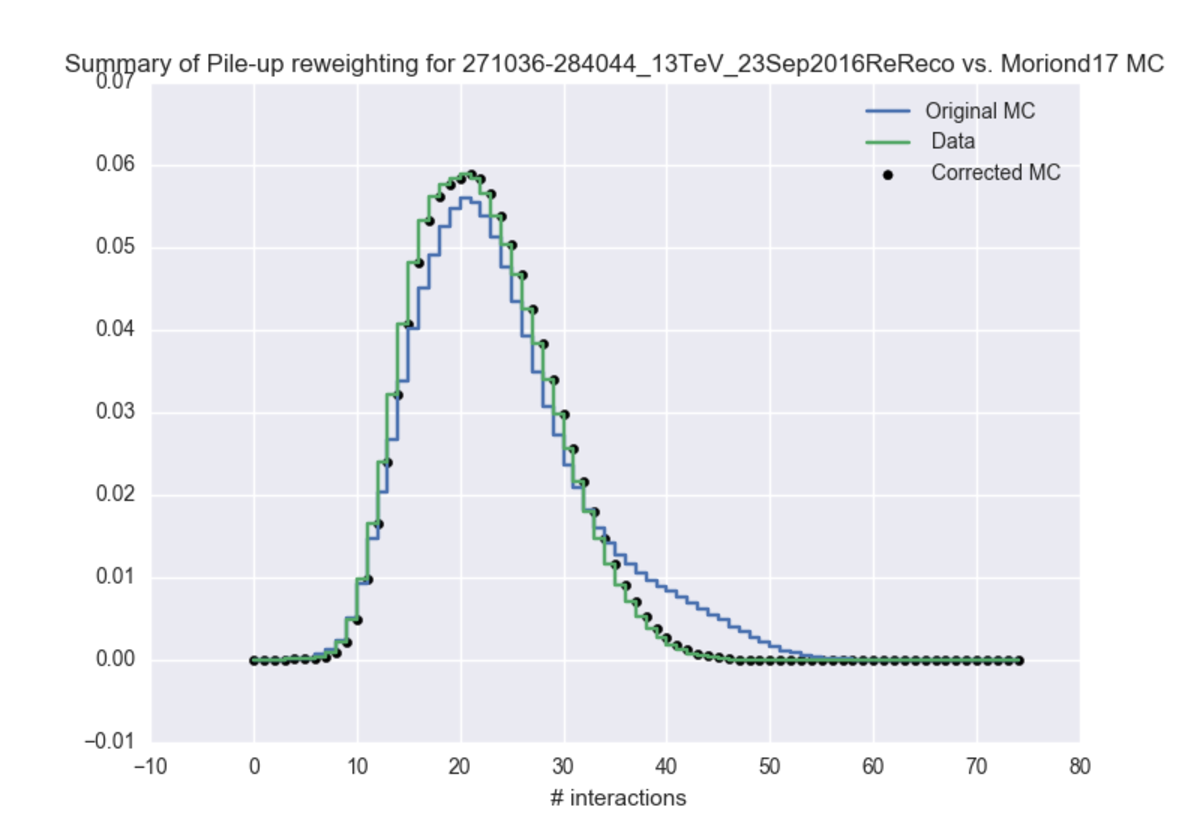
\includegraphics[width=0.5\textwidth]{figures/pileup_reweighting/summarized_data.pdf}} ~
  \subfigure[]{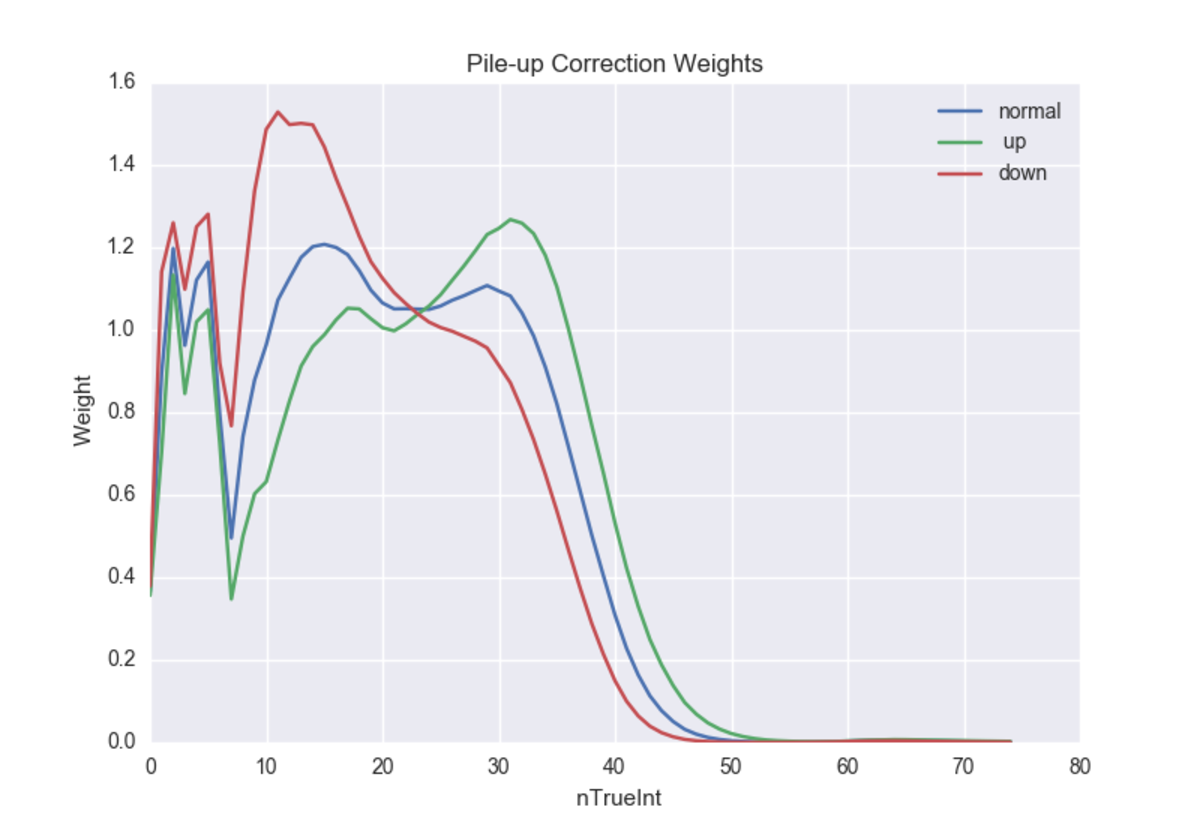
\includegraphics[width=0.5\textwidth]{figures/pileup_reweighting/tbl_20170125_01-tbl_corr_nTrueInt.pdf}} 
  \caption{(a) The distribution of the average numbers of the
    inelastic interactions per colliding bunch pair per lumi section
    in the data, corresponding distribution in the simulated events,
    and that of the reweighted simulated events. (b) The weights
    applied to simulated events as a function of the average number of
    the inelastic interactions per colliding bunch pair per lumi
    section.}
  \label{f044_corr_nTrueInt_data_mc_norm}
\end{figure}

Figure~\ref{f044_corr_nTrueInt_data_mc_norm} shows the distributions
of \verb!nTrueInt! in the data, simulated events and reweighted
simulated events. The figure demonstrates that the simulated events
have the distribution of \verb!nTrueInt! very similar to that found in
the data and after reweighting, the distributions from simulations
from data and simulation are identical.
%We note that the simulation does not contain events with 37 or more
%overlapping pp interactions, while the data do, causing the MC
%weighted distribution not to match perfectly the data. This small
%issue will be recovered once the new MC samples with updated PU
%profile will be available.

\subsubsection{Trigger efficiencies}
\label{sec:trigger-sf}

Simulated events in the signal region are corrected to account for
signal trigger inefficiencies. Simulated events in the muon control
regions rely on the use of an emulated muon trigger and the
application of data/MC scale factors to correct for differences in the
muon trigger efficiencies determined from data and simulation. Further
details are found in Sec.~\ref{sec:triggers}.

\subsubsection{Lepton and photon scale factors}

Simulation mismodelling of efficiencies related to object
identification and isolation requirements are mitigated by the use of
scale factors. Corrections related to trigger and tracking
reconstruction efficiencies are also considered. Typically, the scale
factors are near-unity and are determined by the POGs or the SUSY
lepton scale factor working group. We follow the SUSY Moriond17
recommendations, detailed here~\cite{susymoriond}. Further details are
given in later sections.

\subsubsection{Jet energy scale corrections and b-tag scale factors}
\label{sec:jecs-and-btag-sf}

Jet energy scale corrections and b-tag scale factors are applied to
the simulated event samples following the JetMET and BTV POG
recommendations. Details in subsequent sections. 

\subsubsection{Boson-\texorpdfstring{\Pt}{pT}-dependent NLO corrections}
\label{sec:nlo-intro}

The \MADGRAPH generator is used to simulate W + jets, DY + jets,
\znunu\ + jets, and \gj at leading order. Missing higher order
corrections, which can result in a modified boson \Pt distribution,
can be determined from (QCD) NLO simulation and (EWK) theory
calculations, as done by the the monojet search in the EXO PAG. We
apply these corrections to our simulated samples and assume a 100\%
uncertainty in these corrections, which is propagated through the
analysis and introduced to the likelihood model via a dedicated
nuisance. Further details are given in Secs.~\ref{sec:nlo} and
\ref{sec:nlo-zinv}.

\subsubsection{\texorpdfstring{\nisr}{Nisr} reweighting for \texorpdfstring{\ttbar}{TTbar}}
\label{sec:nisr-intro}
 
To improve on the \MADGRAPH modelling of the multiplicity of
additional jets from initial state radiation (ISR), the SUSY group
recommends to reweight \MADGRAPH \ttbar Monte Carlo events according
to the number of ISR jets (\nisr) identified in the event so as to
improve the jet multiplicity agreement with data. The reweighting
factors vary between 0.92 and 0.51 for $1 \leq \nisr \leq 6$. In this
analysis, we categorise identically the events in the control and
signal regions according to the number of jets reconstructed in an
event. Hence such a correction is expected to have very little impact
on the final result.

Further, this procedure attempts to correct for the mismodelling of
associated jet production for \ttbar processes, which may be due to
missing higher-order calculations in the LO \MADGRAPH MC. Hence, for
consistency with the V + jets samples (also produced with
\MADGRAPH{}@LO), we follow the recommendations of the SUSY group and
apply the \nisr corrections to our simulated samples. The uncertainty
is assumed to be 50\% of the corrections, which is propagated through
the analysis and introduced to the likelihood model via a dedicated
nuisance.

\subsection{Corrections to simulation for signal processes}
\label{sec:signalcorrs}

\fixme{DOCUMENT THE CORRECTIONS TO BE APPLIED!}

%%____________________________________________________________________________||
